\chapter{Análisis de Resultados}

\par En este capitulo se describirá el simulador desarrollado con sus condiciones de diseño, limitaciones, suposiciones, validaciones, funcionalidades y sus posibles usos y aplicaciones.

\section{Horno simulado}

\par El horno escogido es de tipo cabina de simple fuego, con una capacidad de carga de 23 megavatios, o el equivalente aproximado de un cambio de 50 ªC para un flujo de 16 mil metros cúbicos por día de residuo de petroleo con gravedad especifica de 0.84.

\par Estas variables de diseño pueden ser modificados en un futuro pero se tomaron por los datos disponible para comparar contra la simulación.

\subsection{Diseño mecánico}

\par Se puede observar a detalle cada una de las dimensiones en la Figura \ref{apx:img} ampliada en los anexos, estas dimensiones responden a la distribución interna de los tubos para el fluido y sus configuraciones por sección.

\begin{figure}[hbt]
\begin{center}
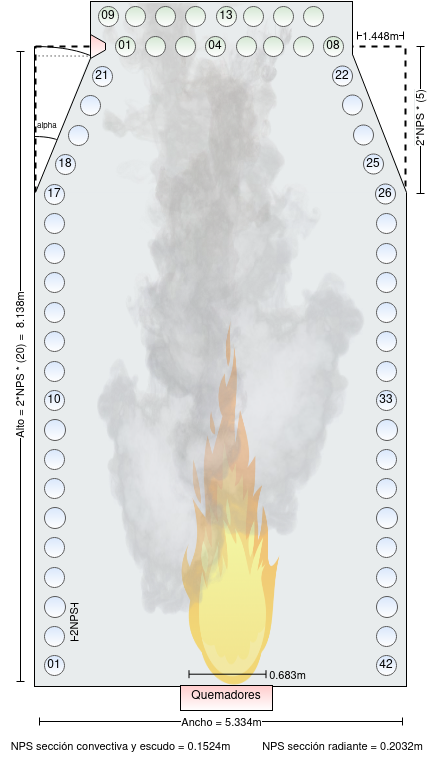
\includegraphics[scale=0.45]{images/firebox}
\caption[Diagrama de la cámara de combustión algoritmo]{Diagrama de la cámara de combustión del horno simulado.}
\label{fig:firebox}
\end{center}
\end{figure}

\par La tabla \ref{tbl:firebox} muestra las dimensiones de la cámara de combustión, mostradas en pies para su correspondiente uso en el cálculo de la longitud promedio de láser, y se pueden denotar los detalles del techo de la cámara en la Figura \ref{fig:firebox}.

\begin{table}
\begin{center}
\caption[Dimensiones de la cámara de combustión]{Dimensiones de la cámara de combustión, mostrada en pies para su uso en la ecuación \ref{eq:pl} y la tabla \ref{tbl:mbl}}
\label{tbl:firebox}
\begin{tabular}{c|c}
Altura interna, ft	& 27.407 \\
Largo interno, ft 	& 64.552 \\
Ancho interno, ft 	& 17.500 \\
\end{tabular}
\end{center}
\end{table}

\par La descripción detallada de las característica de los tubos y aletas usadas se puede encontrar en la tabla \ref{tbl:tubes} y una vista en perspectiva de la distribución de los tubos se puede apreciar en la Figura \ref{fig:diagrama-meca}.

\begin{table}
\begin{center}
\caption[Distribución de tubos en el horno]{Distribución de tubos en el horno}
\label{tbl:tubes}
\begin{tabular}{l|c|c|c}
Sección 					& Radiante			& Escudo			& Convectiva \\
\hline
Material de tubos			& \multicolumn{3}{c}{-- A-312 TP321 --} \\
Soporte de tubos    		& Interno			& Externo			& Externo		\\
Arreglo			    		& Paralelo			& Escalonado		& Escalonado	\\
No. de tubos total    		& 42				& 16				& 40			\\
No. de tubos por fila		& 2					& 8					& 8				\\
Grosor pared de tubos, cm	& 0.818				& 0.711				& 0.711			\\
Di. interno de tubos, cm	& 7.981				& 16.827			& 16.827		\\
Espaciado de tubos, cm  	& 40.640			& 					& 				\\
Espaciado transversal, cm  	&					& 30.480			& 30.480		\\
Espaciado longitudinal, cm 	&					& 30.480			& 30.480		\\
Largo de tubos efectivo, m	& 18.926			& 18.288			& 18.288		\\
\hline
Material de aletas			&					& 					& 11.5-13.5Cr	\\
Tipo de aletas				&					& 					& Solidas		\\	
Altura de aletas, cm		&					& 					& 2.438			\\
Grosor de aletas, cm		&					& 					& 0.152			\\
Densidad de aletas, aleta/m	& 					& 					& 196.850		\\
\end{tabular}
\end{center}
\end{table}

\subsection{Combustible y aire seleccionado}

\par Como combustible se utilizó un gas de refinería por ser lo más común en la industria petrolera, la composición molar establecida para hacer las pruebas del algoritmo se describe en la tabla \ref{tbl:combustible}. Sin embargo, la posibilidad de cambiar la composición esta abierta en la interfaz del simulador.

\par El aire ambiental seco establecido para simplificar los cálculos solo contiene \ac{n2} y \ac{o2}, otros compuestos como el \ac{argon} son despreciados por sus aporte del 1\% o menos a las ecuaciones de combustión. Como se describió en la sección de combustión del capitulo II, la composición tomada para el aire seco es 20.95\% de \ac{o2} y 79.05\% de \ac{n2}.

\par La humedad relativa del aire establecida en las pruebas fue del 50\% con una temperatura ambiente de 26.667 ºC.

\begin{table}
\begin{center}
\caption[Composición del combustible base]{Composición molar porcentual del combustible base.}
\label{tbl:combustible}
\begin{tabular}{l|r}
	Gas combustible					& (Moles \%) \\
	\hline
	Metano ($CH_4$)					& 56.470 \\
	Etano ($C_2H_6$)				& 15.150 \\
	Propano ($C_3H_8$)				& 6.220 \\
	n-Butano ($C_4H_{10}$)			& 1.760 \\
	i-Butano ($C_4H_{10}$)			& 0.750 \\
	Etileno ($C_2H_4$)				& 1.580 \\
	Propileno ($C_3H_6$)			& 2.770 \\
	Monóxido de carbono ($CO$)		& 0.660 \\
	Dióxido de carbono ($CO_2$)		& 2.540 \\
	Hidrógeno ($H_2$)				& 11.420 \\
	Nitrógeno ($N_2$)				& 0.680 \\
	Agua ($H_2O$)					& 0.000 \\
	Oxigeno ($O_2$)					& 0.000 \\
	Sulfuro de hidrógeno ($H_2S$)	& 0.000 \\
\end{tabular}
\end{center}
\end{table}

\subsection{Datos de la combustión}
\par Luego de correr la simulación desarrollada, en la sección de combustión, se obtuvieron los datos de la tabla \ref{tbl:combustion-data}, adicionalmente, la composición del gas de combustión resultante es descrita en la tabla \ref{tbl:combustion-gas}.

\begin{table}
\begin{center}
\caption[Datos de la combustión]{Datos de la combustión, simulador EC 2022 vs WinHeat\copyright}
\label{tbl:combustion-data}
\begin{tabular}{l|c|c}
			& Sim EC 2022 & Winheat \\
	Exceso de aire, \%								& 20.000 & 20.000 \\
	Humedad relativa, \%							& 50.000 & 50.000 \\
	Temperatura del aire, °C						& 26.667 & 26.667 \\
	A/C másica teórica requerido					& 15.574 & 15.577 \\
	A/C másica húmeda con exceso de aire			& 18.689 & 18.693 \\
	Unidad de gas de combustión por unidad de aire  & 19.689 & 19.693 \\
	Poder Calorífico Neto  (NCV), kJ/kg				& 45,718.6 & 45,759.9 \\
	Poder Calorífico Bruto (GCV), kJ/kg				& 50,268.0 & - \\
	Peso Molecular (PM) del combustible, kg/kmol	& 21.149 & - \\
	PM del gas de combustión, kg/kmol				& 27.911 & 27.912 \\
\end{tabular}
\end{center}
\end{table}

\par Para validar la confiabilidad de estos resultados se compararon con los obtenidos en el software privado de diseño de hornos, WinHeat\copyright, con más de 25 años de trayectoria en el mercado, resultados probados en campo y con una subscripción anual valorada en \$4.000.

\par La conclusión de esta comparación arrojó que la diferencia entre los resultados de ambos simuladores es menor al 0.1\% en esta sección.

\begin{table}
\begin{center}
\caption[Composición del gas de combustión]{Composición molar y másica porcentual del gas de combustión}
\label{tbl:combustion-gas}
\begin{tabular}{l|c|c|c}
		& \% Peso & \% Moles (EC 2022)	& \% Moles (WinHeat\copyright) \\
	\hline
	Nitrógeno ($N_2$)			& 72.121	& 71.860	& 71.854	\\
	Oxígeno ($O_2$)				& 3.636 	& 3.172		& 3.172		\\
	Dióxido de carbono ($CO_2$)	& 13.753	& 8.723		& 8.722		\\
	Vapor de agua ($H_2O$)		& 10.490	& 16.245	& 16.252	\\
	Dióxido de azufre ($SO_2$)	& 0.000 	& 0.000		& 0.000		\\
	Monóxido de carbono ($CO$)	& 0.000 	& 0.000		& 0.000		\\
\end{tabular}
\end{center}
\end{table}

\subsection{Datos de la secciones de transferencia de calor}

\par Datos de comparación mostrados en las tablas \ref{tbl:compara-zr}, \ref{tbl:compara-ze} y \ref{tbl:compara-zc}.

\begin{table}
\begin{center}
\caption[Resultados en zona radiante de intercambio de calor]{Comparación de resultados en zona radiante de intercambio de calor.}
\label{tbl:compara-zr}
\begin{tabular}{l|c|c}
	& Sim EC 2022 & WinHeat\copyright \\
Temp. entrada fluido, °C		& 379 & 378	\\
Temp. salida fluido, °C			& 411 & 411	\\
Temp. pared de tubo, °C			& 432 & 459	\\
Temp. salida gas, °C			& 798 & 813	\\

Masa de combustible, kg/s		& 0.574 & 0.564	\\
Calor combustión, MW			& 26.233 & 25.790	\\
Calor aire, MW					& 0.123 & 0.119	\\
Calor combustible, MW			& 0.022 & 0.000	\\

Calor gas de combustión, MW		& 11.083 & 10.615	\\
Calor de perdidas, MW			& 0.393 & 0.226	\\
Calor radiante a escudo, MW		& 1.747 & 1.665	\\
Calor de convección, MW			& 1.705 & 1.650	\\
Calor de radiacion, MW			& 11.443 & 11.753	\\
Calor del fluido, MW			& 13.154 & 13.417	\\

Dist. de calor radiante			& 62.78\% & 64.01\% \\

Área total (At), m$^2$				& 547.09 & 547.01 \\
Área refractaria (Ar), m$^2$		& 566.42 & 541.70 \\
Área de plano frio (Acp), m$^2$		& 323.05 & 369.73 \\
Factor Alpha						& 0.904 & .904 \\

Coef. de conv. int., kJ/h-m$^2$-C	& 2,770.431 & 2,992.684 \\
Coef. de conv. ext., kJ/h-m$^2$-C	& 30.663 & no reporta \\

Longitud media de laser (MBL), ft	& 20.829 & 20.45 \\
P$_{CO^2}$+P$_{H^2O}$, atm 		& 0.249 & 0.250 \\
\end{tabular}
\end{center}
\end{table}

\begin{table}
\begin{center}
\caption[Resultados en zona escudo de intercambio de calor]{Comparación de resultados en zona escudo de intercambio de calor.}
\label{tbl:compara-ze}
\begin{tabular}{l|c|c}
	& Sim EC 2022 & WinHeat\copyright \\
Temp. entrada fluido, °C		& 370 & 369	\\
Temp. salida fluido, °C			& 379 & 378	\\
Temp. pared de tubo, °C			& 401 & 407	\\
Temp. entrada gas, °C			& 798 & 813	\\
Temp. salida gas, °C			& 694 & 674	\\
LMTD, K							& 369.610 & 660.2 \\

Masa gas de combustión, kg/s	& 11.298 & 11.099	\\

Calor gas de combustión, MW		& 1.593 & no reporta \\
Calor de convección, MW			& 1.592 & 1.957	\\
Calor de radiacion, MW			& 1.747 & 1.665	\\
Calor del fluido, MW			& 3.340 & 3.621	\\

Dist. de calor escudo			& 15.89\% &  17.3\% \\

Área total (At), m$^2$				& 154.688 & 158.678 \\
Área de plano frio (Acp), m$^2$		& 44.593 & no reporta \\
Factor Alpha						& 1 & 1 \\

Coef. global de tran. (Uo), kJ/h-m$^2$-C	& 100.253  & 121.016 \\
Coef. de conv. int., kJ/h-m$^2$-C	& 4,426.553 & 4,411.3 \\
Coef. de conv. ext., kJ/h-m$^2$-C	& 30.663 & no reporta \\
\end{tabular}
\end{center}
\end{table}

\begin{table}
\begin{center}
\caption[Resultados en zona convectiva de intercambio de calor]{Comparación de resultados en zona convectiva de intercambio de calor.}
\label{tbl:compara-zc}
\begin{tabular}{l|c|c}
	& Sim EC 2022 & WinHeat\copyright \\
Temp. entrada fluido, °C		& 359 & 369	\\
Temp. salida fluido, °C			& 370 & 370	\\
Temp. pared de tubo, °C			& 366 & 361	\\

Temp. entrada gas, °C			& 694 & 674	\\
Temp. salida gas, °C			& 391 & 382	\\
LMTD, K							& 125.914 & 92 \\  
	t_fin_avg & 366 & 364\\
	t_fin_max & 376 & \\

Calor gas de combustión, MW		& 4.452 & no reporta \\
Calor de convección, MW			& 4.459 & 3.939	\\
Calor del fluido, MW			& 3.340 & 3.621	\\
Calor liberado en chimenea, MW	& 4.910 & no reporta \\

Dist. de calor escudo			& 21.28\% &  18.79\% \\

Área total (At), m$^2$			& 4,670.8 & 4,872.6 \\
Eficiencia de aletas			& 98.77\% & no reporta \\

Coef. global de tran. (Uo), kJ/h-m$^2$-C	& 27.295 & 26.493 \\
Coef. de conv. int., kJ/h-m$^2$-C	& 4,300.2 & 4,331.4 \\
Coef. hr, kJ/h-m$^2$-C			& 1.626 \\
Coef. ho, kJ/h-m$^2$-C			& 27.887 & 35.009 \\
Coef. hc, kJ/h-m$^2$-C			& 26.261 \\
Coef. he, kJ/h-m$^2$-C			& 27.563 & 30.689 \\
\end{tabular}
\end{center}
\end{table}
1.    Ciertamente sería posible considerar todo el algoritmo de cálculo (diseño mecánico del horno y ecuaciones para el desarrollo del Caso Base) como un primer resultado. Podría ser una manera de verlo. 
Este primer resultado debería discutir/comentar, de forma ordenada y secuencial, todas las secciones del cálculo ampliado del Caso Base incluyendo las comparaciones que se hicieron y los porcentajes de error con respecto a las corridas de WinHeat (variables principales). En este grupo también caben las curvas de tendencias, las cuales definen el rango (muchos cálculos) y la confiabilidad (tendencias continuas y sin inestabilidades) del algoritmo
Eso ya lo hiciste mientras discutíamos el algoritmo. 

2.    Adicionalmente habría que considerar también otros "resultados", a saber, aquellos que muestran las prestaciones de la Interfaz (esencialmente las posibilidades educativas que ofrece la comparación de nuevos casos Base y Modificados. 
¿Qué quiero decir con esto?
Que mediante el empleo de ejemplos o "casos de estudio" deberías poder explicar el efecto de ciertas variables (una a la vez, como debe ser) sobre el desempeño del horno tomando como referencia el caso Base, a saber:
-    Efecto de cambios en el flujo de residuo; la diferencia de temperaturas de entrada y salida del residuo; el exceso de aire; el exceso de oxígeno; los factores de ensuciamiento (internos y externos); la temperatura ambiental; la humedad relativa y finalmente el efecto del cambio del combustible. 
-    Quizás podrías combinar en estos ejemplos, el uso de unidades SI en unos e Inglesas en otros. 
-    Cuando digo "discutir", me refiero a explicar el por qué del comportamiento de las variables resultantes. ¿Por qué suben, por qué bajan o por qué no se inmutan? 
Es haciendo esta labor que ejercerías como aspirante al grado de Ing. Químico y no como Ing. de Computación

Al mostrar todas estas comparaciones Caso Base - Caso Modificado estarías abriendo la puerta para que los jurados (y lo usuarios, en general) exploren otras alternativas y, con ello, se eduquen como operadores de hornos.

\section{Interfaz de usuario (UI)}

\subsection{Validación del modelo y tendencias}

3-      El modelo debe ser presentado como una herramienta amplia que está limitado por las características físicas del horno: área de transferencia de calor en las tres zonas de intercambio, capacidad de los quemadores y las dimensiones de la chimenea. Es decir, el diseño mecánico del horno es invariable.

4-      El horno   fue diseñado (dimensionado)  con capacidad de calentamiento para 90.000 BPD de residuo  con un incremento de temperatura desde  632 K a 684 K. Condiciones de diseño.

5-      El modelo permite variar el volumen del fluido del proceso, temperatura de entrada y salida del fluido del proceso, condiciones ambientales, composición del gas de combustión y relación A/C. Las propiedades del fluido, Cp, viscosidad y gravedad específica que utiliza el modelo corresponden a la temperatura de entrada y salida y deben ser introducidas como datos. Las propiedades del gas de combustión son calculadas a partir de sus componentes.

6-      No existe impedimento para variar el fluido del proceso en un amplio margen de crudos con diferentes API u otras corrientes de refinería. Esto debe ser recalcado entre los puntos importantes de las virtudes del modelo.

7-      En forma ilustrativa, se debe mantener el fluido del diseño para demostrar la validez del modelo y  la tendencia de los resultados ante la variación de los parámetros independientes.

8-      Deben quedar claro las limitantes del modelo en aquellos elementos no considerados cuantitativamente (ej. formación de CO, despegue de la llama por exceso de aire, etc) y que han sido tratados mediante rangos empíricos.

\subsection{Aplicaciones}
